\section{Motivation}
Gradual advancement of semiconductor industry continues to reduce chipset cost and power consumption making it possible to embeds more sensors into devices, machines. As a result, estimates have been made that by 2020 there will be 12 billion \ac{M2M} connections globally \cite{machinareport} and 20.8 billion connected devices.\cite{Gartner} 

With such technological advancement another revolution in the industry is foreseen,
which will also influence the global GDP (Figure~\ref{img:gdp}). If industry/factories are running many machines that are connected to different kind of sensors, all the data that this sensors generate are very costly to move to cloud. Running applications that uses this sensor data in a Fog node will reduce the cost.

\begin{figure}[H]
  \centering
  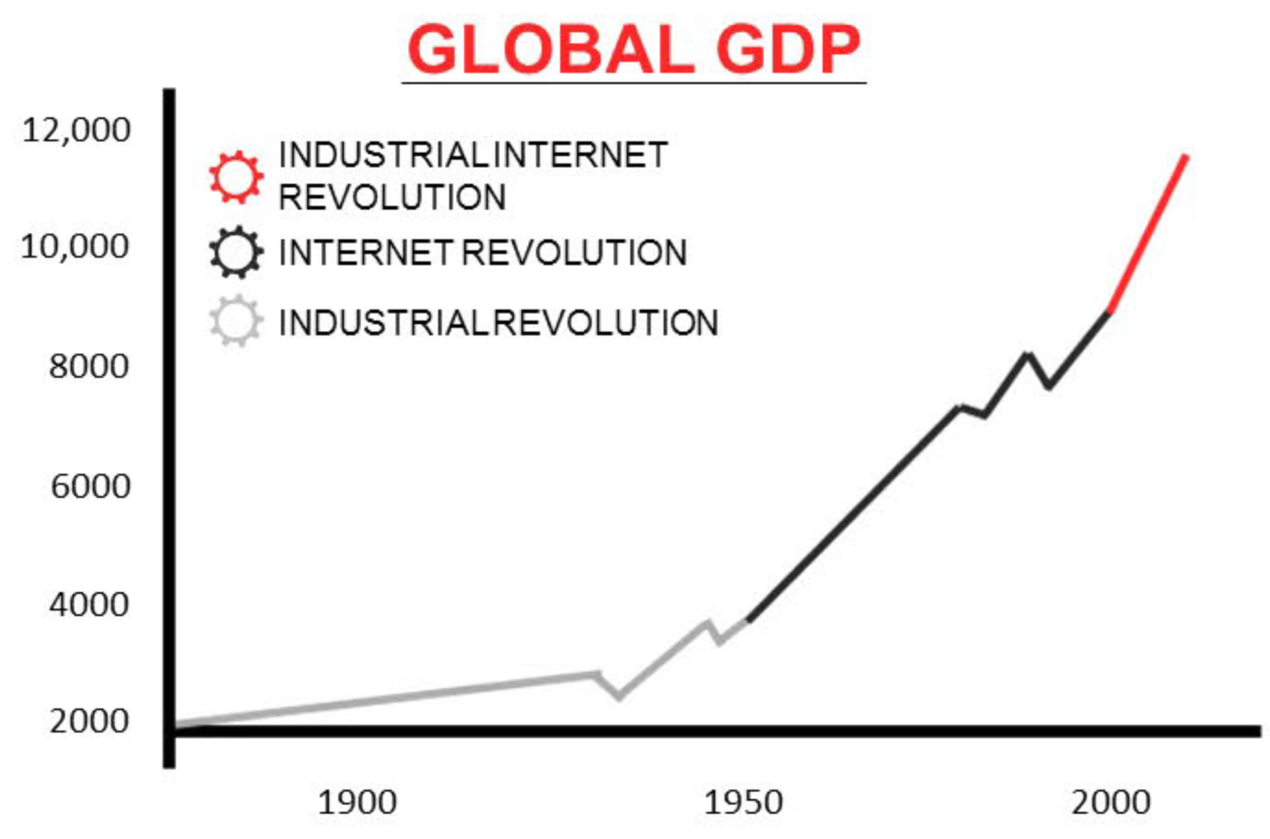
\includegraphics[width=.55\textwidth]{img/gdp}
  \caption{Expected Influence with IoT implementations (ERS International Macroeconomic Data Set)}\label{img:gdp}
\end{figure}

The sensors embedded with these billions of Internet of Things (IoT) \cite{Alberti2013} devices will gather data from even
more physical assets. This will generate big data.

According to the 2014 annual report on Big Data by EMC and IDC, predictions
are that, by 2020 the connectable assets will generate about 44 ZB(1 ZB = 1 billion TB) of data. To deal with the Big
Data challenge in the field of IoT FOG node (A machine that runs IoT application locally) has emerged which has gotten a lot of attention recently.

We are implementing a FOG node, that can run any IoT applications. Now, if the sensors are generating huge data, all the data trasferring to cloud, and saving in cloud is highly expensive. Whereas, running in fog node will reduce the cost significantly. 